\documentclass[10pt]{beamer}

\usetheme{Madrid}
\usecolortheme{default}
\setbeamertemplate{navigation symbols}{}
\setbeamersize{text margin left=0.6cm,text margin right=0.6cm}

\usepackage{tikz}
\usetikzlibrary{automata, positioning, arrows.meta, shapes.geometric, calc}
\usepackage{amsmath, amssymb}
\pdfstringdefDisableCommands{\def\translate#1{#1}}

\title{Regular Expressions and Regular Grammars}
\subtitle{Algebraic Descriptions and Grammatical Foundations}
\author[SDB]{}
\date{\scriptsize \textit{Theory of Computation Slide Sets}}

\begin{document}

\begin{frame}
  \titlepage
\end{frame}

\begin{frame}{Table of Contents}
  \tableofcontents
\end{frame}

\begin{frame}{Learning Outcomes}
  By the end of this slide set, you should be able to:
  \begin{itemize}
    \item interpret a regular expression as a language and apply precedence
      rules correctly;
    \item convert a regular expression to an equivalent $\varepsilon$-NFA;
    \item convert a finite automaton to a regular expression by state
      elimination;
    \item recognize right-linear and left-linear grammars and convert between
      regular grammars and finite automata;
    \item justify conversions using a path/derivation invariant; and
    \item distinguish a grammar's syntactic form from its language's class.
  \end{itemize}
\end{frame}

% ==========================================
% Part 1: Regular Expressions (RE)
% ==========================================
\section{Regular Expressions (RE)}

\begin{frame}{Part 1: Inductive Definition of RE}
  \small

  Regular expressions (REs) provide a declarative, algebraic way to describe languages. We define them inductively based on the regular operations.
  \pause

  \begin{block}{Formal Definition}
    Given an alphabet $\Sigma$, $R$ is a regular expression if $R$ is built by
    the following rules, and no others. Its denoted language is written $L(R)$.
  \begin{enumerate}\setlength\itemsep{1pt}
      \item $a$ for $a \in \Sigma$, with $L(a)=\{a\}$;
      \item $\varepsilon$, with $L(\varepsilon)=\{\varepsilon\}$;
      \item $\emptyset$, with $L(\emptyset)=\emptyset$;
      \item $(R_1 \cup R_2)$, with $L(R_1\cup R_2)=L(R_1)\cup L(R_2)$;
      \item $(R_1 \circ R_2)$, with $L(R_1\circ R_2)=L(R_1)L(R_2)$;
      \item $(R_1^*)$, with $L(R_1^*)=[L(R_1)]^*$.
    \end{enumerate}
  \end{block}
  \pause
  \begin{exampleblock}{Notation Note}
    We use $\cup$ for union and $\varepsilon$ for the empty string. Some texts instead use $+$ for union and $\lambda$ for the empty string.
    Here $R^+=RR^*$ abbreviates one or more repetitions; this superscript
    $+$ is not union.
  \end{exampleblock}
\end{frame}

\begin{frame}{Precedence Rules and Empty-Language Notation}
  To avoid excessively nested parentheses, we establish an order of operations:
  \begin{center}
    \textbf{Star ($*$) \quad $>$ \quad Concatenation ($\circ$) \quad $>$ \quad Union ($\cup$)}
  \end{center}
  For example, $0 \cup 10^*$ is parsed as $0 \cup (1 \circ (0^*))$, not $(0 \cup 1) \circ 0^*$.
  \pause
  \vspace{0.25cm}

  \begin{alertblock}{Teacher's Corner: $\emptyset$ vs. $\{\varepsilon\}$}
    A frequent source of confusion is the distinction between the expressions
    $\emptyset$ and $\varepsilon$ and the languages they denote.
    \begin{itemize}
      \item $L(\emptyset)=\emptyset$ contains \textbf{no strings}.
      \item $L(\varepsilon)=\{\varepsilon\}$ contains \textbf{exactly one
        string}: the empty string.
      \item Concatenation identities: $R\varepsilon\equiv R$, but
        $R\emptyset\equiv\emptyset$, where $\equiv$ means equal languages.
      \item Union identities: $R\cup\emptyset\equiv R$; $R\cup\varepsilon$
        ensures that the empty string is included (it may already be present).
    \end{itemize}
  \end{alertblock}
\end{frame}

\begin{frame}{Useful Algebraic Laws for Regular Expressions}
  \small
  These are language equivalences: $R\equiv S$ means $L(R)=L(S)$.
  \begin{columns}[T]
    \column{0.48\textwidth}
    \begin{block}{Identity and Annihilation}
      \[
        \begin{aligned}
          R\cup\emptyset&\equiv R,& R\cup R&\equiv R,\\
          R\varepsilon&\equiv\varepsilon R\equiv R,\\
          R\emptyset&\equiv\emptyset R\equiv\emptyset.
        \end{aligned}
      \]
    \end{block}
    \column{0.48\textwidth}
    \begin{block}{Star and Distribution}
      \[
        \begin{aligned}
          \emptyset^*&\equiv\varepsilon,& \varepsilon^*&\equiv\varepsilon,\\
          R(S\cup T)&\equiv RS\cup RT,\\
          (R\cup S)T&\equiv RT\cup ST.
        \end{aligned}
      \]
    \end{block}
  \end{columns}
  \begin{alertblock}{Important Non-Law}
    Concatenation is not commutative in general: $ab\not\equiv ba$.
    These laws simplify state-elimination labels and help check answers.
  \end{alertblock}
\end{frame}

\begin{frame}{Examples of Regular Expressions}
  \small
  Let $\Sigma = \{0, 1\}$. How do we express common patterns algebraically?
  \pause

  \vspace{0.3cm}
  \textbf{1. Strings containing at least one $00$ as a substring:}
  \[ (0 \cup 1)^{*} 00 (0 \cup 1)^{*} \]
  \textit{Explanation:} The $(0 \cup 1)^{*}$ acts as a wildcard $\Sigma^*$ representing any prefix and any suffix.
  \pause

  \vspace{0.3cm}
  \textbf{2. Strings that do not contain $00$ as a substring:}
  \[ (1 \cup 01)^{*}(0 \cup \varepsilon) \]
  \textit{Explanation:} Every nonfinal $0$ is followed by a $1$; at most one
  unmatched $0$ may occur, and only at the end.
  \pause

  \vspace{0.3cm}
  \textbf{3. Strings with an even number of 0s:}
  \[ 1^* (01^*01^*)^{*} \]
  \textit{Explanation:} 1s can appear anywhere. 0s must appear in pairs ($01^*0$) to ensure their total count is even.
\end{frame}

\begin{frame}{Prove the Pattern, Not Just the Examples}
  \small
  Why does $R=(1\cup01)^*(\varepsilon\cup0)$ describe exactly the binary
  strings with no occurrence of $00$?
  \begin{block}{Soundness: every generated word has the property}
    Each repeated block is $1$ or $01$, so it ends in $1$. Joining such
    blocks never creates $00$; the optional final $0$ cannot do so either.
  \end{block}
  \pause
  \begin{block}{Completeness: every valid word is generated}
    Scan a word with no $00$ from left to right. Take each $1$ as a block;
    pair each nonfinal $0$ with its following $1$ to make $01$. If a final
    $0$ remains, use the optional ending. These blocks form an $R$-word.
  \end{block}
  \pause
  \textbf{Boundary tests:} $\varepsilon,0,1,010$ must be included;
  $00,1001$ must be excluded. Tests catch errors, but the two inclusions
  establish correctness for every length.
\end{frame}

% ==========================================
% Part 2: RE to NFA (Thompson's Construction)
% ==========================================
\section{RE to NFA (Thompson Construction)}

\begin{frame}{Part 2: RE to NFA --- Thompson's Construction}
  \textbf{Kleene's Theorem:} A language is regular if and only if it is
  described by a regular expression.

  Here we prove the direction \emph{regular expression $\Rightarrow$ regular
  language} by converting any RE into an equivalent $\varepsilon$-NFA. First,
  we establish the atomic primitives:
  \pause
  \vspace{0.3cm}

  \begin{columns}
    \column{0.33\textwidth}
    \centering \textbf{RE: $a$ for $a \in \Sigma$} \\
    \vspace{0.2cm}
    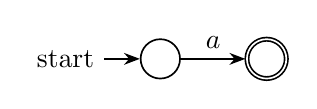
\begin{tikzpicture}[->, >=Stealth, auto, node distance=1.35cm, semithick]
      \node[state, initial, inner sep=2pt, minimum size=0.5cm] (s) {};
      \node[state, accepting, inner sep=2pt, minimum size=0.5cm] (e) [right of=s] {};
      \path (s) edge node {$a$} (e);
    \end{tikzpicture}

    \column{0.33\textwidth}
    \pause
    \centering \textbf{RE: $\varepsilon$} \\
    \vspace{0.2cm}
    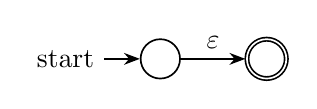
\begin{tikzpicture}[->, >=Stealth, auto, node distance=1.35cm, semithick]
      \node[state, initial, inner sep=2pt, minimum size=0.5cm] (s) {};
      \node[state, accepting, inner sep=2pt, minimum size=0.5cm] (e) [right of=s] {};
      \path (s) edge node {$\varepsilon$} (e);
    \end{tikzpicture}

    \column{0.33\textwidth}
    \pause
    \centering \textbf{RE: $\emptyset$} \\
    \vspace{0.2cm}
    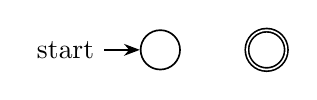
\begin{tikzpicture}[->, >=Stealth, auto, node distance=1.35cm, semithick]
      \node[state, initial, inner sep=2pt, minimum size=0.5cm] (s) {};
      \node[state, accepting, inner sep=2pt, minimum size=0.5cm] (e) [right of=s] {};
    \end{tikzpicture}
  \end{columns}
  \vspace{0.5cm}
  \begin{center}
    Each primitive has one start state and one distinct accept state; the $\emptyset$ machine simply has no path between them.
  \end{center}
\end{frame}

\begin{frame}{Inductive Steps: Union and Concatenation}
  \small
  Use disjoint copies of the Thompson fragments for $R_1$ and $R_2$.
  Each box's left boundary is its entry; its right boundary is its exit.
  \pause
  \begin{columns}
    \column{0.5\textwidth}
    \textbf{Union ($R_1 \cup R_2$)}
    \begin{center}
      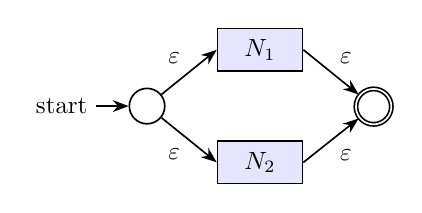
\begin{tikzpicture}[->, >=Stealth, auto, node distance=1.2cm, semithick, scale=0.9, transform shape]
        \node[state, initial, inner sep=1pt, minimum size=0.5cm] (s) {};
        \node[draw, rectangle, minimum width=1.2cm, minimum height=0.6cm, fill=blue!10] (m1) [above right=0.3cm and 0.8cm of s] {$N_1$};
        \node[draw, rectangle, minimum width=1.2cm, minimum height=0.6cm, fill=blue!10] (m2) [below right=0.3cm and 0.8cm of s] {$N_2$};
        \node[state, accepting, inner sep=1pt, minimum size=0.5cm] (f) [below right=0.3cm and 0.8cm of m1] {};

        \path (s) edge node[above left] {$\varepsilon$} (m1.west)
        (s) edge node[below left] {$\varepsilon$} (m2.west)
        (m1.east) edge node[above right] {$\varepsilon$} (f)
        (m2.east) edge node[below right] {$\varepsilon$} (f);
      \end{tikzpicture}
    \end{center}

    \column{0.5\textwidth}
    \pause
    \textbf{Concatenation ($R_1 \circ R_2$)}
    \begin{center}
      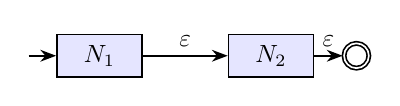
\begin{tikzpicture}[->, >=Stealth, auto, node distance=1.5cm, semithick, scale=0.9, transform shape]
        \node[draw, rectangle, minimum width=1.2cm, minimum height=0.6cm, fill=blue!10] (m1) {$N_1$};
        \node[draw, rectangle, minimum width=1.2cm, minimum height=0.6cm, fill=blue!10] (m2) [right=1.2cm of m1] {$N_2$};

        \draw[->] (-1, 0) -- (m1.west);
        \draw[->] (m1.east) -- node {$\varepsilon$} (m2.west);
        \node[state, accepting, minimum size=0.35cm, inner sep=0pt]
          (exit) [right=0.4cm of m2] {};
        \draw[->] (m2.east) -- node[above] {$\varepsilon$} (exit);
      \end{tikzpicture}
    \end{center}
  \end{columns}
  \vspace{0.3cm}
  In the combined machine, internal fragment exits lose their accepting
  status; only the overall exit accepts. The displayed extra final state
  for concatenation is optional. All joining edges consume no input.
\end{frame}

\begin{frame}{Inductive Steps: The Star Operation}
  \textbf{Star Operation ($R_1^*$)}
  \vspace{0.2cm}

  The Star operation requires us to accept the empty string $\varepsilon$ (zero repetitions), or loop back to the beginning of $N_1$ after a successful pass (one or more repetitions).
  \pause
  \begin{center}
    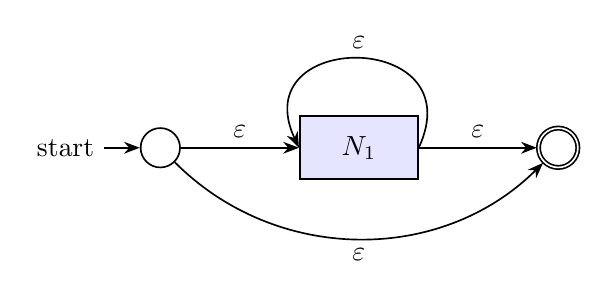
\begin{tikzpicture}[->, >=Stealth, auto, node distance=2cm, semithick]
      \node[state, initial, inner sep=1pt, minimum size=0.5cm] (s) {};
      \node[draw, rectangle, minimum width=1.5cm, minimum height=0.8cm, fill=blue!10] (m1) [right=1.5cm of s] {$N_1$};
      \node[state, accepting, inner sep=1pt, minimum size=0.5cm] (f) [right=1.5cm of m1] {};

      \path (s) edge node {$\varepsilon$} (m1.west)
      (m1.east) edge node {$\varepsilon$} (f)
      (s) edge[bend right=45] node[below] {$\varepsilon$} (f);

      \draw[->] (m1.east) to[out=65,in=115,looseness=2.8]
        node[above] {$\varepsilon$} (m1.west);
    \end{tikzpicture}
  \end{center}
  \pause
  \textit{Why new boundary states?} The new start has no incoming transitions and the new accept has no outgoing transitions. This preserves the one-entry/one-exit form needed by later inductive steps.
\end{frame}

\begin{frame}{Worked Example: Converting
  \texorpdfstring{$(ab \cup a)^{*}$}{(ab union a)*}}
  \small
  Let's build an NFA for $(ab \cup a)^{*}$ stage-by-stage.
  \pause

  \textbf{1. Build separate primitives for the two occurrences of $a$ and for $b$.}
  \pause

  \textbf{2. Concatenate them to obtain $ab$:}
  \begin{center}
    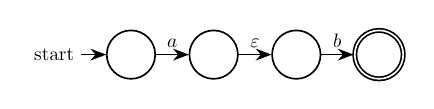
\begin{tikzpicture}[->, >=Stealth, auto, node distance=1.5cm, semithick, scale=0.7, transform shape]
      \node[state, initial] (1) {};
      \node[state] (2) [right of=1] {};
      \node[state] (3) [right of=2] {};
      \node[state, accepting] (4) [right of=3] {};
      \path (1) edge node {$a$} (2) (2) edge node {$\varepsilon$} (3) (3) edge node {$b$} (4);
    \end{tikzpicture}
  \end{center}
  \pause

  \textbf{3. Form $U=(ab \cup a)$:}
  \begin{center}
    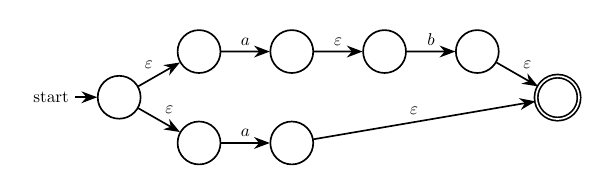
\begin{tikzpicture}[->, >=Stealth, auto, node distance=1.2cm, semithick, scale=0.62, transform shape]
      \node[state, initial] (s) {};
      \node[state] (t1) [above right=0.3cm and 1cm of s] {};
      \node[state] (t2) [right=1cm of t1] {};
      \node[state] (t3) [right=1cm of t2] {};
      \node[state] (t4) [right=1cm of t3] {};
      \node[state] (b1) [below right=0.3cm and 1cm of s] {};
      \node[state] (b2) [right=1cm of b1] {};
      \node[state, accepting] (f) [below right=0.3cm and 1cm of t4] {};

      \path (s) edge node {$\varepsilon$} (t1) (s) edge node {$\varepsilon$} (b1)
      (t1) edge node {$a$} (t2) (t2) edge node {$\varepsilon$} (t3) (t3) edge node {$b$} (t4)
      (b1) edge node {$a$} (b2)
      (t4) edge node {$\varepsilon$} (f) (b2) edge node {$\varepsilon$} (f);
    \end{tikzpicture}
  \end{center}
\end{frame}

\begin{frame}{Worked Example: Star Wrapper and a Check}
  \small
  Recall the one-entry/one-exit fragment $U$ for $ab\cup a$.
  \textbf{4. Apply the star wrapper to $U$:}
  \begin{center}
    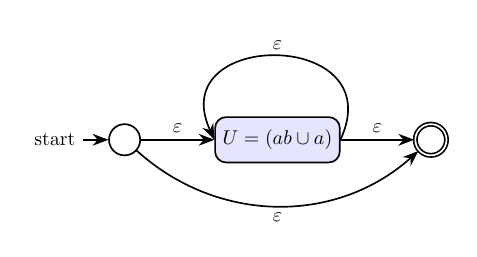
\begin{tikzpicture}[->, >=Stealth, auto, semithick, scale=0.72, transform shape]
      \node[state, initial, minimum size=0.55cm] (s0) {};
      \node[draw, rounded corners, minimum width=2.2cm, minimum height=0.8cm,
      fill=blue!10, right=1.3cm of s0] (u) {$U=(ab\cup a)$};
      \node[state, accepting, minimum size=0.55cm, right=1.3cm of u] (f0) {};
      \path (s0) edge node {$\varepsilon$} (u.west)
      (u.east) edge node {$\varepsilon$} (f0)
      (s0) edge[bend right=42] node[below] {$\varepsilon$} (f0);
      \draw (u.east) to[out=65,in=115,looseness=2.5]
        node[above] {$\varepsilon$} (u.west);
    \end{tikzpicture}
  \end{center}
  \pause
  \begin{columns}[T]
    \column{0.53\textwidth}
    \begin{block}{Trace the choices}
    $\varepsilon$ takes the bypass. The word $abaab$ is accepted as
    $(ab)(a)(ab)$: enter $U$ three times, using its exit-to-entry edge between
    repetitions. The word $abb$ cannot be partitioned into $a$ or $ab$ blocks.
    \end{block}
    \column{0.43\textwidth}
    \centering
    \textbf{Equivalent compact NFA}\\
    (not a Thompson fragment)
    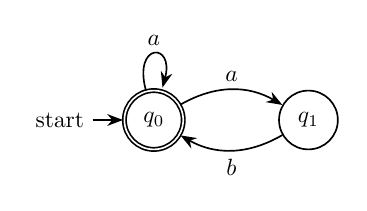
\begin{tikzpicture}[->,>=Stealth,node distance=1.4cm,semithick,
      scale=0.85,transform shape]
      \node[state,initial,accepting] (ready) {$q_0$};
      \node[state,right=of ready] (pending) {$q_1$};
      \path (ready) edge[loop above] node[above] {$a$} (ready)
        (ready) edge[bend left] node[above] {$a$} (pending)
        (pending) edge[bend left] node[below] {$b$} (ready);
    \end{tikzpicture}
  \end{columns}
\end{frame}

% ==========================================
% Part 3: FA to RE (The State Elimination Method)
% ==========================================
\section{FA to RE (State Elimination)}

\begin{frame}{Part 3: Generalized NFAs (GNFA)}
  To convert a finite automaton back into a regular expression, we use a
  \textbf{generalized NFA (GNFA)}.
  \pause
  \begin{block}{What is a GNFA?}
    A GNFA has transition arrows labeled by \textbf{regular expressions}
    rather than single symbols. Traversing an edge consumes any string in the
    language denoted by its label.
  \end{block}
  \pause
  \textbf{Standard Form for GNFA conversion:}
  \begin{enumerate}
    \item A new \textbf{start state} with an $\varepsilon$-arrow to the old start state, and no incoming arrows.
    \item A single new \textbf{accept state} with $\varepsilon$-arrows from the old accept states, and no outgoing arrows.
    \item Combine parallel arrows by union and regard a missing arrow as one
      labeled $\emptyset$. Thus each allowable ordered pair has one RE label;
      the start has no incoming arrows and the accept state has no outgoing
      arrows.
  \end{enumerate}
\end{frame}

\begin{frame}{The Conversion Algorithm: State Elimination}
  \small
  \textbf{Objective:} Reduce the machine to two states (start and accept) by
  eliminating internal states one at a time.
  \pause

  When we eliminate a state $q_r$, we update the graph so that its language
  remains unchanged. To compute the new label on $q_i\rightarrow q_j$:
  \pause

  \begin{center}
    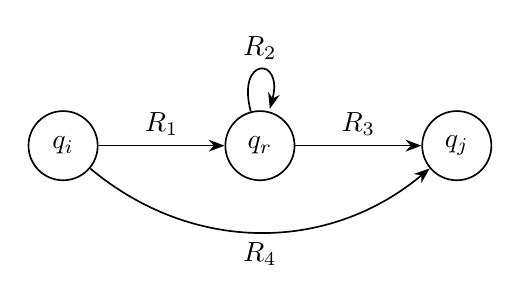
\begin{tikzpicture}[->, >=Stealth, auto, node distance=2.5cm, semithick]
      \node[state] (qi) {$q_i$};
      \node[state] (qrip) [right of=qi] {$q_r$};
      \node[state] (qj) [right of=qrip] {$q_j$};

      \path (qi) edge node {$R_1$} (qrip)
      (qrip) edge [loop above] node {$R_2$} (qrip)
      (qrip) edge node {$R_3$} (qj)
      (qi) edge [bend right=40] node [below] {$R_4$} (qj);
    \end{tikzpicture}
  \end{center}
  \pause
  \begin{block}{The Update Formula}
    The new label bypassing $q_r$ from $q_i$ to $q_j$ becomes:
    \[ R' = R_4 \cup R_1R_2^*R_3 \]
    Use the \textbf{old labels} for every allowable pair of remaining states,
    including self-loops ($q_i=q_j$). Different orders may produce different-looking but
    equivalent expressions.
  \end{block}
\end{frame}

\begin{frame}{Worked Example: DFA to GNFA}
  \textbf{Given DFA:} Accepts strings with an odd number of 1s.
  \begin{center}
    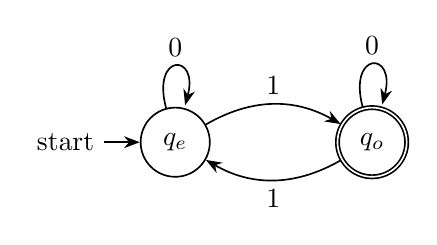
\begin{tikzpicture}[->, >=Stealth, auto, node distance=2.5cm, semithick]
      \node[state, initial] (qe) {$q_e$};
      \node[state, accepting] (qo) [right of=qe] {$q_o$};
      \path (qe) edge [bend left] node {$1$} (qo)
      (qe) edge [loop above] node {$0$} (qe)
      (qo) edge [bend left] node {$1$} (qe)
      (qo) edge [loop above] node {$0$} (qo);
    \end{tikzpicture}
  \end{center}
  \pause

  \textbf{Step 1: Convert to Standard GNFA} (Add new start $s$ and accept $a$).
  \begin{center}
    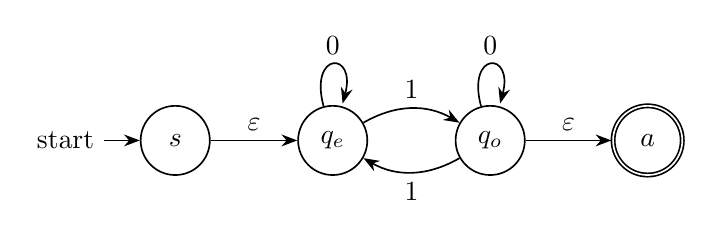
\begin{tikzpicture}[->, >=Stealth, auto, node distance=2cm, semithick]
      \node[state, initial] (s) {$s$};
      \node[state] (qe) [right of=s] {$q_e$};
      \node[state] (qo) [right of=qe] {$q_o$};
      \node[state, accepting] (a) [right of=qo] {$a$};

      \path (s) edge node {$\varepsilon$} (qe)
      (qe) edge [bend left] node {$1$} (qo)
      (qe) edge [loop above] node {$0$} (qe)
      (qo) edge [bend left] node {$1$} (qe)
      (qo) edge [loop above] node {$0$} (qo)
      (qo) edge node {$\varepsilon$} (a);
    \end{tikzpicture}
  \end{center}
\end{frame}

\begin{frame}{Worked Example: State Elimination}
  \small
  \textbf{Step 2: Eliminate $q_o$.} 
  
  Update the labels on
  $q_e\rightarrow q_e$ and $q_e\rightarrow a$.
  \begin{itemize}
    \item $q_e\rightarrow q_e$: the bypass through $q_o$ contributes
      $10^*1$. Union with the existing $0$ to obtain $0\cup10^*1$.
    \item $q_e\rightarrow a$: the bypass contributes
      $10^*\varepsilon=10^*$. Union with $\emptyset$ to obtain $10^*$.
  \end{itemize}
  \pause
  \begin{center}
    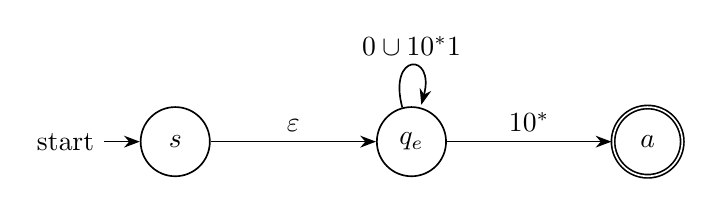
\begin{tikzpicture}[->, >=Stealth, auto, node distance=3cm, semithick]
      \node[state, initial] (s) {$s$};
      \node[state] (qe) [right of=s] {$q_e$};
      \node[state, accepting] (a) [right of=qe] {$a$};

      \path (s) edge node {$\varepsilon$} (qe)
      (qe) edge [loop above] node {$0 \cup 10^*1$} (qe)
      (qe) edge node {$10^*$} (a);
    \end{tikzpicture}
  \end{center}
  \pause
  \textbf{Step 3: Eliminate $q_e$.}
  
  Now we update the edge $s \rightarrow a$.
  
  Path: $s \xrightarrow{\varepsilon} q_e
  \xrightarrow{(0 \cup 10^*1)^{*}} q_e \xrightarrow{10^*} a$.

  \vspace{0.2cm}
  \textbf{Final RE:} $(0 \cup 10^*1)^{*}10^*$.
  Every repeated block contributes zero or two $1$'s; the final $10^*$
  contributes one. Pairing the first $2k$ ones in any odd-parity word shows
  completeness. An alternative is $0^*1(0^*10^*1)^*0^*$.
\end{frame}

% ==========================================
% Part 4: Regular Grammars
% ==========================================
\section{Regular Grammars}

\begin{frame}{Grammar Notation and Language Generation}
  \small
  We use the Linz-style order $G=(V,T,S,P)$:
  \begin{itemize}
    \item $V$: a finite set of variables (nonterminals);
    \item $T$: a finite terminal alphabet, disjoint from $V$;
    \item $S\in V$: the start variable;
    \item $P$: finitely many productions $A\to\alpha$, with $A\in V$ and
      $\alpha\in(V\cup T)^*$, restricted further on the next slide.
  \end{itemize}
  \pause
  A step replaces one variable using a production:
  \[
    uAv\Rightarrow u\alpha v\quad\text{if }A\to\alpha\in P.
  \]
  $\Rightarrow^*$ means zero or more steps, and
  \[
    L(G)=\{w\in T^*:S\Rightarrow^*w\}.
  \]
  A terminal-only result is a completed word; $aS$ is not one.
  $A\to x\mid y$ abbreviates two productions, not a terminal bar.
\end{frame}

\begin{frame}{Part 4: Definitions of Regular Grammars}
  \small    

  We have seen that DFAs, NFAs, and REs all describe regular languages. We can
  also define this class syntactically using restricted grammars.
  \pause

  \begin{block}{Regular Grammar Definition}
    A grammar $G = (V, T, S, P)$ is \textbf{regular} if all of its productions
    are right-linear or all of its productions are left-linear.
    In both definitions below, $A,B\in V$ and $x\in T^*$.

    \textbf{Right-Linear:} All productions are of the form:
    \begin{itemize}
      \item $A \rightarrow xB$ \quad ($A, B \in V$, $x \in T^*$)
      \item $A \rightarrow x$
    \end{itemize}

    \textbf{Left-Linear:} All productions are of the form:
    \begin{itemize}
      \item $A \rightarrow Bx$
      \item $A \rightarrow x$
    \end{itemize}
  \end{block}
  \pause
  \textit{Important:} At most one variable appears on each right-hand side,
  and its orientation must be consistent throughout the grammar. Having at
  most one variable is necessary, but not sufficient, for a grammar to be
  regular. We allow $x=\varepsilon$, hence unit rules $A\to B$ and
  terminating rules $A\to\varepsilon$; some texts use a stricter convention.
\end{frame}

\begin{frame}{Right-Linear, Left-Linear, or Merely Linear?}
  \small
  \begin{columns}[T]
    \column{0.48\textwidth}
    \begin{block}{Right-linear example}
      \[
        S \rightarrow abS \mid a
      \]
      Every variable is at the right end. The generated language is
      \[
        L=(ab)^{*}a.
      \]
    \end{block}

    \column{0.48\textwidth}
    \begin{block}{Left-linear example}
      \[
        \begin{aligned}
          S&\rightarrow Aab,\\
          A&\rightarrow Aab \mid B,\\
          B&\rightarrow a.
        \end{aligned}
      \]
      Every variable is at the left end. Here
      $L=aab(ab)^{*}$.
    \end{block}
  \end{columns}
  \pause
  \begin{alertblock}{Do Not Mix the Two Orientations}
    The grammar with rules $S\rightarrow aA$, $A\rightarrow Sb$, and
    $S\rightarrow\varepsilon$ is linear but not a regular grammar: it mixes
    right- and left-linear productions. In fact, it generates the nonregular
    language $\{a^n b^n:n\geq 0\}$.
  \end{alertblock}
  This is a restriction on the \emph{grammar}. A mixed grammar may still
  generate a regular language; its form alone does not decide that question.
\end{frame}

\begin{frame}{Reading Derivations in a Regular Grammar}
  Consider the right-linear grammar
  \[
    S\rightarrow abS \mid a.
  \]
  \pause
  Each use of $S\rightarrow abS$ contributes one block $ab$ and keeps the
  derivation active. The rule $S\rightarrow a$ terminates it.
  \begin{exampleblock}{Sample Derivations}
    \[
      \begin{aligned}
        S &\Rightarrow a,\\
        S &\Rightarrow abS \Rightarrow aba,\\
        S &\Rightarrow abS \Rightarrow ababS \Rightarrow ababa.
      \end{aligned}
    \]
  \end{exampleblock}
  \pause
  Thus every completed derivation has the form $(ab)^{n}a$, and every
  $(ab)^{n}a$ can be derived. Therefore $L(G)=(ab)^{*}a$.
\end{frame}

\begin{frame}{Normalizing Long Terminal Blocks}
  Some definitions permit productions $A\rightarrow xB$ and $A\rightarrow x$
  with $x\in T^*$. Before drawing an NFA, split each long terminal block into
  one-symbol steps.
  \pause
  \begin{block}{General Replacement}
    For $k\geq2$, replace
    \[
      A\rightarrow a_1a_2\cdots a_kB
    \]
    by fresh variables $C_1,\ldots,C_{k-1}$ and rules
    \[
      A\rightarrow a_1C_1,\quad
      C_1\rightarrow a_2C_2,\quad\ldots\quad,
      C_{k-1}\rightarrow a_kB.
    \]
    For a terminal-only rule $A\rightarrow a_1\cdots a_k$, use the same chain
    but end with $C_{k-1}\rightarrow a_k$ (or a transition to the new final
    state in the NFA construction).
  \end{block}
  \pause
  \begin{exampleblock}{Example}
    With fresh $V_2$, $V_1\rightarrow abV_0$ becomes
    $V_1\rightarrow aV_2$ and $V_2\rightarrow bV_0$.
    The introduced variable records progress through the terminal block.
  \end{exampleblock}
\end{frame}

\begin{frame}{Theorem: Right-Linear Grammar to NFA}
  \small
  \begin{block}{Theorem}
    If $G=(V,T,S,P)$ is right-linear, then $L(G)$ is a regular language.
  \end{block}
  \pause
  \textbf{Construction after normalizing terminal blocks:}
  \begin{enumerate}
    \item Use one state for each variable and make $S$ the start state.
    \item For $A\rightarrow aB$, add the transition $A\xrightarrow{a}B$.
    \item For $A\rightarrow B$, add $A\xrightarrow{\varepsilon}B$.
    \item For $A\rightarrow a$, add $A\xrightarrow{a}F$ to one new accept
      state $F$.
    \item For $A\rightarrow\varepsilon$, either make $A$ accepting or add
      $A\xrightarrow{\varepsilon}F$.
  \end{enumerate}
  \pause
  \begin{exampleblock}{Why the Construction Works}
    In the normalized grammar, $S\Rightarrow^*wA$ exactly when there is a
    path to variable-state $A$ labeled $w$ (ignoring $\varepsilon$-moves).
    Reaching an accept state corresponds precisely to
    completing a derivation $S\Rightarrow^*w$.
  \end{exampleblock}
\end{frame}

\begin{frame}{Worked Example: Regular Grammar to NFA}
  \small
  Consider
  \[
    S\rightarrow aS\mid bA,
    \qquad
    A\rightarrow aA\mid a.
  \]
  \pause
  \begin{center}
    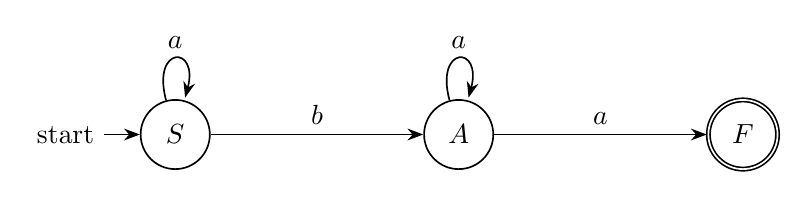
\begin{tikzpicture}[->, >=Stealth, auto, node distance=2.7cm, semithick]
      \node[state, initial] (S) {$S$};
      \node[state, right=of S] (A) {$A$};
      \node[state, accepting, right=of A] (F) {$F$};
      \path (S) edge[loop above] node {$a$} (S)
      (S) edge node {$b$} (A)
      (A) edge[loop above] node {$a$} (A)
      (A) edge node {$a$} (F);
    \end{tikzpicture}
  \end{center}
  \pause
  \begin{columns}[T]
    \column{0.48\textwidth}
    \textbf{Derivation}
    \[
      \begin{aligned}
        S&\Rightarrow aS\Rightarrow aaS\Rightarrow aabA\\
        &\Rightarrow aabaA\Rightarrow aabaa.
      \end{aligned}
    \]
    \column{0.48\textwidth}
    \textbf{Language}
    \[
      L(G)=a^*ba^+=a^*baa^*.
    \]
  \end{columns}
\end{frame}

\begin{frame}{Theorem: NFA to Right-Linear Grammar}
  \small
  \begin{block}{Theorem}
    If $L\subseteq\Sigma^*$ is regular, then some right-linear grammar
    $G=(V,\Sigma,S,P)$ satisfies $L=L(G)$.
  \end{block}
  \pause
  Let $M=(Q,\Sigma,\delta,q_0,F)$ be an NFA for $L$.
  \begin{enumerate}
    \item Create one variable $Q_i$ for every automaton state $q_i$.
    \item Use $Q_0$ as the grammar's start variable.
    \item For each transition $q_i\xrightarrow{a}q_j$, add
      $Q_i\rightarrow aQ_j$.
    \item For each $\varepsilon$-transition $q_i\xrightarrow{\varepsilon}q_j$, add
      $Q_i\rightarrow Q_j$.
    \item For every accepting state $q_f$, add $Q_f\rightarrow\varepsilon$.
  \end{enumerate}
  \pause
  A path labeled $w$ from $q_0$ to $q_f$ corresponds step-for-step to a
  derivation $Q_0\Rightarrow^*wQ_f\Rightarrow w$.
\end{frame}

\begin{frame}{Worked Example: DFA to Right-Linear Grammar}
  \small
  The DFA below accepts exactly the binary strings ending in $01$.
  \begin{center}
    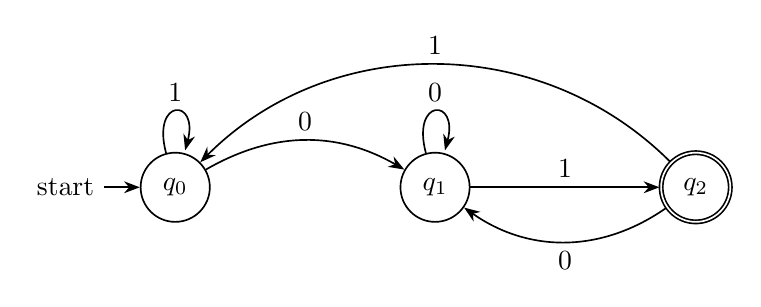
\begin{tikzpicture}[->, >=Stealth, auto, node distance=2.4cm, semithick]
      \node[state, initial] (q0) {$q_0$};
      \node[state, right=of q0] (q1) {$q_1$};
      \node[state, accepting, right=of q1] (q2) {$q_2$};
      \path (q0) edge[bend left] node {$0$} (q1)
      (q0) edge[loop above] node {$1$} (q0)
      (q1) edge[loop above] node {$0$} (q1)
      (q1) edge node {$1$} (q2)
      (q2) edge[bend left=35] node[below] {$0$} (q1)
      (q2) edge[bend right=45] node[above] {$1$} (q0);
    \end{tikzpicture}
  \end{center}
  \pause
  Replace states by variables $Q_0,Q_1,Q_2$:
  \[
    \begin{aligned}
      Q_0&\rightarrow 0Q_1\mid 1Q_0,\\
      Q_1&\rightarrow 0Q_1\mid 1Q_2,\\
      Q_2&\rightarrow 0Q_1\mid 1Q_0\mid\varepsilon.
    \end{aligned}
  \]
\end{frame}

\begin{frame}{Left-Linear Grammars and the Equivalence Theorem}
  \small
  \begin{block}{Left-Linear Version}
    A language is regular if and only if it is generated by a left-linear grammar.
  \end{block}
  \pause
  For a finite automaton, build productions in the reverse direction:
  \begin{itemize}
    \item If $q_i\xrightarrow{a}q_j$, add $Q_j\rightarrow Q_i a$.
    \item If $q_i\xrightarrow{\varepsilon}q_j$, add $Q_j\rightarrow Q_i$.
    \item Introduce a new grammar start $S$ with $S\rightarrow Q_f$ for each
      accepting state $q_f$.
    \item Add $Q_0\rightarrow\varepsilon$ for the automaton's start state.
  \end{itemize}
  \pause
  \begin{block}{Combined Equivalence}
    For every language $L$, the following are equivalent:
    \begin{align*}
      L\text{ is regular}
      &\Longleftrightarrow L=L(G_R)\text{ for some right-linear }G_R\\
      &\Longleftrightarrow L=L(G_L)\text{ for some left-linear }G_L.
    \end{align*}
  \end{block}
\end{frame}

\begin{frame}{Regular-Grammar Checkpoint Exercises}
  \small
  \begin{enumerate}
    \item Classify each \emph{grammar} as right-linear, left-linear, linear
      but not a regular grammar, or not linear:
      \begin{enumerate}
        \item $S\rightarrow 0S\mid 1A$, $A\rightarrow 1$;
        \item $S\rightarrow A0$, $A\rightarrow A1\mid\varepsilon$;
        \item $S\rightarrow 0A$, $A\rightarrow S1\mid\varepsilon$.
      \end{enumerate}
    \item Convert $S\rightarrow 0S\mid 1A$, $A\rightarrow 0A\mid 1$
      into an NFA and describe its language.
    \item Construct a right-linear grammar for all binary strings that end in
      $00$.
  \end{enumerate}
  \pause
  \begin{alertblock}{Proof Practice}
    State the invariant that connects a partial derivation $S\Rightarrow^*wA$
    with a path in the corresponding NFA.
  \end{alertblock}
\end{frame}

% ==========================================
% Part 5: The "Big Picture" & Applications
% ==========================================
\section{The Big Picture \& Applications}

\begin{frame}{Part 5: The Equivalence Map}
  Four formalisms describe exactly the regular languages.
  \pause

  \begin{center}
    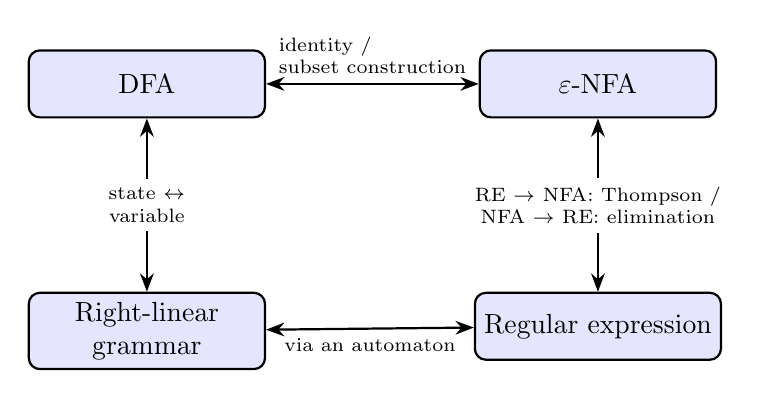
\begin{tikzpicture}[
        box/.style={draw, rounded corners, minimum width=3.0cm, minimum height=0.85cm,
        fill=blue!10, thick, align=center},
      link/.style={<->, >=Stealth, thick}, node distance=2.2cm and 2.7cm]
      \node[box] (DFA) {DFA};
      \node[box, right=of DFA] (NFA) {$\varepsilon$-NFA};
      \node[box, below=of DFA] (RG) {Right-linear\\grammar};
      \node[box, below=of NFA] (RE) {Regular expression};

      \draw[link] (DFA) -- node[above, font=\scriptsize, align=left] {identity /\\subset construction} (NFA);
      \draw[link] (NFA) -- node[midway, fill=white, font=\scriptsize, align=center]
        {RE $\to$ NFA: Thompson /\\NFA $\to$ RE: elimination} (RE);
      \draw[link] (DFA) -- node[midway, fill=white, font=\scriptsize, align=center]
        {state $\leftrightarrow$\\variable} (RG);
      \draw[link] (RG) -- node[below, font=\scriptsize] {via an automaton} (RE);
    \end{tikzpicture}
  \end{center}
\end{frame}

\begin{frame}{Applications of Regular Languages}
  Why do we care about regular expressions and finite automata?
  \pause

  \begin{block}{1. Compiler Design (Lexical Analysis)}
    Compilers use regular expressions to define the tokens of a programming
    language (e.g., identifiers, constants, and reserved words).

    If $D=(0\cup\cdots\cup9)$, a simple signed decimal can be described by
    $(\varepsilon\cup\texttt{+}\cup\texttt{-})DD^*(\varepsilon\cup\texttt{.}DD^*)$.
    Tools such as \texttt{lex} convert token specifications into efficient
    finite-automaton-based scanners.
  \end{block}
  \pause

  \begin{block}{2. Pattern Matching and Text Editors}
    For an RE of syntax-tree size $m$ and an input of length $n$, Thompson-NFA
    simulation takes $O(mn)$ time and $O(m)$ working space. For a fixed RE,
    this is linear in $n$. A prebuilt DFA needs $O(n)$ matching time, but
    constructing it can require exponentially many states.
  \end{block}
\end{frame}

% ==========================================
% Pedagogical Enhancements
% ==========================================
\section{Review and Exercises}

\begin{frame}{Checkpoint Exercises}
  \begin{enumerate}
    \item \textbf{GNFA Conversion:} Given a DFA that accepts strings ending in
      $1$, with states $q_0$ (start) and $q_1$ (accept), the transitions are
      $\delta(q_0,0)=q_0$, $\delta(q_0,1)=q_1$,
      $\delta(q_1,0)=q_0$, and $\delta(q_1,1)=q_1$.

      Convert this DFA to a regular expression using state elimination.

      \vspace{0.6cm}
    \item \textbf{Grammars:} Write a right-linear grammar for the language:
      \[ L = \{w \in \{0,1\}^* \mid w \text{ ends in } 01 \}. \]
  \end{enumerate}
\end{frame}

\begin{frame}{Practice: Design, Explain, and Find a Counterexample}
  \small
  Work over $\Sigma=\{0,1\}$ unless stated otherwise.
  \begin{enumerate}
    \item Give an RE for exactly two $1$'s. Explain why it permits all
      positions of the $0$'s but no third $1$.
    \item Give an RE for words in which every maximal run of $0$'s has even
      length. Is that the same as having an even total number of $0$'s?
    \item Disprove $(R\cup S)^*\equiv R^*\cup S^*$ with concrete
      expressions and a distinguishing word.
    \item A student converts $S\to aS\mid\varepsilon$ into an automaton
      containing only an $a$-loop at a nonaccepting start state. What is missing?
  \end{enumerate}
  \pause
  \begin{block}{Discuss before opening the appendix answers}
    Check $\varepsilon$ and the shortest examples first. Then justify every
    accepted word, not merely a few test cases.
  \end{block}
\end{frame}

\begin{frame}{Summary: One Class, Several Useful Representations}
  \small
  \begin{itemize}
    \item REs describe languages using union, concatenation, and star;
      an expression is syntax, while $L(R)$ is its meaning.
    \pause
    \item Thompson's construction proves RE $\Rightarrow$ finite automaton
      by structural induction and one-entry/one-exit fragments.
    \pause
    \item State elimination proves the converse by preserving path languages
      while deleting internal states.
    \pause
    \item Right-linear grammars follow accepting paths forwards; left-linear
      grammars can reconstruct the same paths backwards.
    \pause
    \item Equal expressive power does not imply equal representation size,
      and a syntactically nonregular grammar may still generate a regular
      language.
  \end{itemize}
  \begin{block}{Bridge to Slide Set 4}
    These constructions become tools for proving closure, deciding questions
    about regular languages, and identifying the limits of finite memory.
  \end{block}
\end{frame}

\appendix
\section{Appendix: Further Constructions and Worked Solutions}

\begin{frame}{Appendix Guide: Choose a Route}
  \small
  The main lecture ends at the summary. This appendix keeps optional depth
  available without interrupting the core conversion methods.
  \begin{block}{Moved out of the main lecture}
    Empty-string tests; detailed Thompson and state-elimination proofs;
    the left-linear converse; programming-regex caveats; extra conversion
    practice; and checkpoint answers.
  \end{block}
  \begin{block}{Suggested enrichment routes}
    \begin{itemize}
      \item \textbf{Exam preparation:} practice solutions and worked challenges.
      \item \textbf{Algebra:} RE identities, Arden's lemma, and grammar equations.
      \item \textbf{Implementation:} derivatives and position automata.
    \end{itemize}
  \end{block}
  Problems with textbook attributions are adapted and solved here; the
  additional extensions are original practice. Closure, decision properties,
  and the pumping lemma are left to Slide Set~4.
\end{frame}

\subsection{Supplementary Explanations}

\begin{frame}{Shorthand, Membership, and the Empty String}
  \small
  Abbreviations do not add expressive power:
  \[
    R^+=RR^*,\qquad R?=(R\cup\varepsilon),\qquad
    R^0=\varepsilon,\quad R^{k+1}=R^kR.
  \]
  Here the superscript $+$ means one or more repetitions, not union.
  Each occurrence of $R$ may contribute a different word of $L(R)$.
  \pause
  \begin{block}{Does an expression accept the empty string?}
    Write $\nu(R)$ for the truth value of $\varepsilon\in L(R)$. Then
    \[
      \begin{aligned}
        \nu(a)&=\nu(\emptyset)=\mathrm{false},&
        \nu(\varepsilon)&=\mathrm{true},\\
        \nu(R\cup S)&=\nu(R)\lor\nu(S),&
        \nu(RS)&=\nu(R)\land\nu(S),\\
        \nu(R^*)&=\mathrm{true}.&&
      \end{aligned}
    \]
  \end{block}
  \pause
  Thus $R^+$ can contain $\varepsilon$ if $R$ does. In this course,
  membership matches the \emph{whole word}; a substring search for $R$
  instead asks for membership in $\Sigma^*L(R)\Sigma^*$.
\end{frame}

\begin{frame}{Why Thompson's Construction Works}
  \small
  \begin{block}{Structural-induction invariant}
    The fragment $N_R$ has distinct entry and exit states, no edge entering
    its entry or leaving its exit, and accepts exactly $L(R)$.
    These boundary conditions hold before the fragment is embedded.
  \end{block}
  \pause
  \begin{itemize}
    \item \textbf{Atoms:} the three primitive diagrams have the required
      languages $\{a\}$, $\{\varepsilon\}$, and $\emptyset$.
    \item \textbf{Union:} every successful path uses one selected branch.
    \item \textbf{Concatenation:} every successful path splits into a path
      through $N_{R_1}$ followed by a path through $N_{R_2}$.
    \item \textbf{Star:} every successful path traverses the body zero or
      more times, yielding a finite concatenation of words of $L(R)$.
  \end{itemize}
  \pause
  Conversely, each such choice of words gives a successful path. Thus the
  induction proves equality, not just inclusion. For an RE syntax tree of
  size $m$, the construction uses $O(m)$ states and transitions; it need not
  give the smallest NFA or DFA.
\end{frame}

\begin{frame}{Why State Elimination Preserves the Language}
  \small
  \begin{block}{Path invariant}
    Each label summarizes paths of one or more edges between its endpoints
    whose internal states have already been eliminated. Initially, labels summarize the original
    edges; after eliminating $q_r$, paths may also pass through $q_r$.
  \end{block}
  \pause
  A path between remaining states either avoids $q_r$, contributing
  $R_{ij}$, or enters it, loops there any finite number of times, and leaves:
  \[
    R'_{ij}=R_{ij}\cup R_{ir}(R_{rr})^*R_{rj}.
  \]
  Conversely, every word in this new label expands into an old path.
  \pause
  \begin{alertblock}{Important edge cases}
    If $q_r$ has no loop, $R_{rr}=\emptyset$ but $(R_{rr})^*=\varepsilon$:
    passing through once is still possible. If no accepting path exists,
    the final label is $\emptyset$. If the old start accepts, the new
    $s$-to-$f$ path preserves acceptance of $\varepsilon$.
  \end{alertblock}
  When only $s$ and $f$ remain, their label denotes the original language.
\end{frame}

\begin{frame}{Left-Linear Conversion: Direction Matters}
  \small
  For the automaton with start $q_0$, loop $q_0\xrightarrow{a}q_0$, and
  transition $q_0\xrightarrow{b}q_1$ to its sole accepting state, use
  \[
    S\to Q_1,\qquad Q_1\to Q_0b,\qquad
    Q_0\to Q_0a\mid\varepsilon.
  \]
  For example,
  \[
    S\Rightarrow Q_1\Rightarrow Q_0b\Rightarrow Q_0ab
      \Rightarrow Q_0aab\Rightarrow aab.
  \]
  We reconstruct the path backwards, but the terminal word is still in its
  original order. Both descriptions give $a^*b$.
  \pause
  \begin{block}{Converse: why every left-linear grammar is regular}
    Reverse every production's right side: $A\to Bx$ becomes
    $A\to x^RB$, and $A\to x$ becomes $A\to x^R$. The resulting
    right-linear grammar generates $L(G)^R$, which is regular. Reversing an
    NFA's edges and exchanging its initial/final boundaries recognizes the
    reversal; thus $L(G)$ is regular too.
  \end{block}
\end{frame}

\begin{frame}{Classical REs Versus Programming Regex}
  \small
  \begin{block}{Notation is not computational power}
    Character classes, optional pieces, and bounded repetitions are shorthand
    for finite unions and concatenations. They remain regular. Backtracking
    is an implementation strategy, not a new language operation: it can be
    slow even for a classical regular expression.
  \end{block}
  \pause
  \begin{exampleblock}{Backreferences really can go beyond regularity}
    Under whole-string matching, the programming pattern
    \texttt{([01]*)\char92{}1} requires two identical binary halves.
    It denotes $\{ww:w\in\{0,1\}^*\}$, which is not regular.
    The symbol \texttt{\char92{}1} is not an operator in our RE definition.
  \end{exampleblock}
  \pause
  Do not classify every lookaround as nonregular: assertions built only from
  regular subpatterns can express regular constraints. Separate the
  \emph{language described} from the \emph{engine's running time}.
\end{frame}

\subsection{Practice and Solutions}

\begin{frame}{Hints: Regular-Grammar Checkpoint}
  \small
  \begin{block}{Hints}
    \begin{itemize}
      \item Exercise 1(a): right-linear, language $0^*11$.
        Exercise 1(b): left-linear, language $1^*0$.
        Exercise 1(c): mixed linear, language
        $\{0^{n+1}1^n:n\ge0\}$, since $S\Rightarrow0S1$ or $S\Rightarrow0$.
      \item For Exercise 2, use states $S$, $A$, and a new final state $F$.
        The resulting regular expression is $0^*10^*1$.
      \item Exercise 3: $S\to0S\mid1S\mid0A$, $A\to0B$,
        $B\to\varepsilon$. Guess the beginning of the final $00$.
    \end{itemize}
  \end{block}
  \pause
  \begin{exampleblock}{Invariant for the Proof}
    For every $w\in T^*$ and $A\in V$,
    \[
      S\Rightarrow^*wA
      \quad\Longleftrightarrow\quad
      \text{the normalized construction has a path }S\xrightarrow{w}A.
    \]
  \end{exampleblock}
\end{frame}

\begin{frame}{Hints for Checkpoint Exercises}
  \begin{block}{Hints}
    \begin{itemize}
      \item \textbf{Exercise 1:}
        \begin{itemize}
          \item Add the standard GNFA start ($s$) and accept ($a$) states.
          \item When ripping $q_1$, the path $q_0 \rightarrow q_1 \rightarrow q_0$ creates a loop on $q_0$ labeled $11^*0$.
          \item The total loop on $q_0$ becomes $0 \cup 11^*0$.
          \item The path to $a$ is via $q_1 \rightarrow a$ which is $\varepsilon$, so $q_0 \rightarrow q_1 \rightarrow a$ gives $11^*$.
          \item Eliminating $q_0$ next gives
            $(0\cup11^*0)^{*}11^*$, which is equivalent to
            $(0\cup1)^{*}1$.
        \end{itemize}
      \item \textbf{Exercise 2:} One answer is
        $S\rightarrow0S\mid1S\mid0A$, $A\rightarrow1B$, and
        $B\rightarrow\varepsilon$. The nondeterministic choice on $0$ guesses
        the start of the final suffix $01$.
    \end{itemize}
  \end{block}
  \pause
  \begin{alertblock}{Final Pro-Tip for State Elimination}
    Simplify regular-expression labels after each state-elimination update.
    For instance, replace $\varepsilon R$ by $R$ and $R\cup\emptyset$ by $R$.
    This keeps the final expression readable and easier to verify.
  \end{alertblock}
\end{frame}

\begin{frame}{Solutions: Design and Counterexamples}
  \small
  \begin{enumerate}
    \item Exactly two $1$'s: $0^*10^*10^*$. The two literal $1$'s are
      separated and surrounded by arbitrary $0$-blocks.
    \pause
    \item Even $0$-runs: $(1\cup00)^*$. Every run is a concatenation of
      $00$ blocks, and any even run can be divided into such blocks.
      The word $010$ has even total zero count but two odd runs, so the
      conditions differ.
    \pause
    \item Let $R=0$, $S=1$. The word $01$ is in $L((0\cup1)^*)$ but
      not in $L(0^*\cup1^*)$. Star of a union allows mixed factors.
    \pause
    \item Make the start state accepting, or add an $\varepsilon$-edge to
      a fresh accepting state. The omitted rule $S\to\varepsilon$ supplies
      termination, including acceptance of the empty word.
  \end{enumerate}
\end{frame}

\begin{frame}{Practice: Conversion and Grammar Structure}
  \small
  \begin{enumerate}
    \item Over $\{a,b,c\}$, classify
      $S\to aA$, $A\to Bb$, $B\to c$. Is its generated language regular?
    \item Normalize $S\to abS\mid\varepsilon$ and draw an equivalent NFA.
      Explain why the variable introduced for $ab$ must be fresh.
    \item A GNFA has $s\xrightarrow{a}r$, $r\xrightarrow{b}f$, and
      $s\xrightarrow{c}f$, with no loop on $r$. Eliminate $r$.
    \item Construct both a right-linear and a left-linear grammar for
      $a^*b$. Give one derivation of $aab$ in each.
  \end{enumerate}
  \pause
  \begin{alertblock}{What a complete conversion answer includes}
    Identify the start and accepting states or start variable, list all rules
    or transitions, and state the path/derivation invariant. A correct-looking
    diagram alone does not explain correctness.
  \end{alertblock}
\end{frame}

\begin{frame}{Solutions: Conversion and Grammar Structure}
  \small
  \begin{enumerate}
    \item The grammar is linear but mixes orientations. Its only terminal
      derivation is $S\Rightarrow aA\Rightarrow aBb\Rightarrow acb$.
      The singleton language $\{acb\}$ is regular.
    \pause
    \item Use $S\to aC\mid\varepsilon$, $C\to bS$, with fresh $C$.
      The NFA has accepting start $S$, an $a$-edge to $C$, and a $b$-edge
      back to $S$. Reusing an existing variable could introduce unintended
      choices midway through the block.
    \pause
    \item The new label is $c\cup a\emptyset^*b\equiv c\cup ab$.
      No loop means zero repetitions, not the absence of a bypass path.
    \pause
    \item Right-linear: $S\to aS\mid b$, with
      $S\Rightarrow aS\Rightarrow aaS\Rightarrow aab$.
      Left-linear: $S\to Ab$, $A\to Aa\mid\varepsilon$, with
      $S\Rightarrow Ab\Rightarrow Aab\Rightarrow Aaab\Rightarrow aab$.
  \end{enumerate}
\end{frame}

\subsection{Algebraic Methods}

\begin{frame}{More RE Laws: Useful but Easy to Misapply}
  \small
  In addition to associativity and commutativity of union, and associativity
  of concatenation, the following are valid language equivalences:
  \[
    \begin{aligned}
      R^*&\equiv\varepsilon\cup RR^*
          \equiv\varepsilon\cup R^*R,\\
      (R^*)^*&\equiv R^*,\qquad R^*R^*\equiv R^*,\\
      (R\cup S)^*&\equiv R^*(SR^*)^*.
    \end{aligned}
  \]
  \pause
  \textbf{Proof idea for the last identity:} group any sequence of $R$- and
  $S$-factors into an initial run of $R$-factors followed by zero or more
  groups consisting of one $S$-factor and a run of $R$-factors.
  Conversely, such groups are sequences of $R$- and $S$-factors.
  \pause
  \begin{alertblock}{Do not distribute star over union or concatenation}
    $(R\cup S)^*\not\equiv R^*\cup S^*$ in general, and
    $(RS)^*\not\equiv R^*S^*$ in general. For $R=a$, $S=b$, the word $a$
    distinguishes $(ab)^*$ from $a^*b^*$.
  \end{alertblock}
\end{frame}

\begin{frame}{Arden's Lemma: An Algebraic Alternative}
  \small
  Here $A,B,X$ denote \emph{languages}, not grammar variables.
  \begin{block}{Arden's Lemma}
    $X=AX\cup B$ always has the least solution $X=A^*B$.
    If $\varepsilon\notin A$, that solution is unique.
  \end{block}
  \pause
  \textbf{Proof sketch.} Substitution verifies that $A^*B$ is a solution.
  Any solution contains $B,AB,A^2B,\ldots$, hence contains $A^*B$.
  If $\varepsilon\notin A$, each recursive factor from $A$ consumes at
  least one symbol, so repeatedly decomposing a finite word of $X$ must
  reach $B$. Thus $X\subseteq A^*B$ too.
  \pause
  \begin{alertblock}{Order and the hypothesis both matter}
    For $X=XA\cup B$, the least solution is $BA^*$.
    With $A=\{\varepsilon\}$ and $B=\emptyset$, the equation becomes $X=X$:
    every language is a solution, so uniqueness fails.
  \end{alertblock}
\end{frame}

\begin{frame}{Worked Language Equations: Odd Number of Ones}
  \small
  Let $X_e$ and $X_o$ be the languages accepted starting from the even and
  odd states of the earlier parity DFA. Decompose by the first transition:
  \[
    X_e=0X_e\cup1X_o,\qquad
    X_o=\varepsilon\cup0X_o\cup1X_e.
  \]
  Only the accepting state contributes $\varepsilon$.
  \pause
  Applying Arden's lemma to the second equation gives
  \[
    X_o=0^*(\varepsilon\cup1X_e).
  \]
  Substitute into the first equation and distribute:
  \[
    X_e=(0\cup10^*1)X_e\cup10^*.
  \]
  \pause
  The coefficient language excludes $\varepsilon$, so Arden gives
  \[
    X_e=(0\cup10^*1)^*10^*,
  \]
  exactly the expression obtained by eliminating the odd state first.
\end{frame}

\subsection{Worked Design and Conversion Challenges}

\begin{frame}{Challenge: Exactly One Occurrence of 00}
  \small
  \textbf{Task.} Design a binary RE with exactly one occurrence of $00$,
  counting overlapping occurrences. Thus $000$ has two and must be rejected.
  \pause
  \begin{exampleblock}{Solution}
    \[
      (1\cup01)^*\,00\,(1\cup10)^*.
    \]
  \end{exampleblock}
  \textbf{Soundness.} The prefix has no $00$ and is empty or ends in $1$.
  The suffix has no $00$ and is empty or starts in $1$. Therefore the
  displayed middle pair is the only occurrence, including at the joins.
  \pause
  \textbf{Completeness.} Split a valid word around its unique $00$. Its
  prefix and suffix must have exactly those boundary restrictions; factor
  them into $1/01$ blocks and $1/10$ blocks, respectively.
  \begin{alertblock}{The tempting wrong answer}
    $(0\cup1)^*00(0\cup1)^*$ guarantees \emph{at least} one occurrence,
    not exactly one. Test $00$, $10010$, $000$, and $00100$.
  \end{alertblock}
  {\scriptsize Original worked exercise in the RE-design style of Linz,
  Chapter~3, and Sipser, Section~1.3.}
\end{frame}

\begin{frame}{Challenge: Binary Numbers at Least 40}
  \small
  \textbf{Task.} Describe binary representations of integers at least $40$.
  Allow leading zeros; the empty word is not a representation here.
  Let $B=(0\cup1)$, and let $B^k$ mean $k$ concatenated copies.
  \pause
  \begin{exampleblock}{Split by significant length}
    \[
      0^*\bigl(1B^6B^*\;\cup\;1(01\cup10\cup11)B^3\bigr).
    \]
  \end{exampleblock}
  \begin{itemize}
    \item At least seven significant bits: the value is at least $64$.
      These words are $1B^6B^*$.
    \pause
    \item Six significant bits: $40=101000_2$. The admissible first three
      bits are $101$, $110$, or $111$; the last three bits are arbitrary.
    \pause
    \item At most five significant bits: the value is at most $31$.
      These words are excluded. An initial $0^*$ does not change the value.
  \end{itemize}
  \textbf{Boundary checks:} reject $100111$ ($39$), accept $101000$ ($40$)
  and $00101000$, and accept $1000000$ ($64$).
  \par\smallskip
  {\scriptsize Textbook-style numerical RE challenge; the case analysis
  and leading-zero convention are made explicit here.}
\end{frame}

\begin{frame}{Sipser Challenge: Constrained Positions}
  \small
  \textbf{Task.} Over $\{0,1\}$, require a $1$ at every odd-numbered
  position, counting from position~1. The empty word satisfies the condition.
  \pause
  Group positions into pairs, with a possible final odd position:
  \[
    \bigl(1(0\cup1)\bigr)^*(\varepsilon\cup1).
  \]
  Every pair starts with $1$; conversely, every valid word has this pairing.
  \pause
  \begin{block}{Harder extension: also require an even number of zeros}
    Write $U=11$ and $V=10$ for the two pair types. Only a $V$ contributes
    a zero, so pair the $V$-blocks:
    \[
      U^*(VU^*VU^*)^*(\varepsilon\cup1).
    \]
    The optional final $1$ does not change the zero count.
  \end{block}
  {\scriptsize Base problem adapted from Sipser's Exercise~1.18,
  as identified in the course assignment~\cite{sheard}; the even-zero
  strengthening and solutions are original.}
\end{frame}

\begin{frame}{Sipser Challenge: RE to a Compact NFA}
  \small
  \textbf{Task.} Build an NFA, then a DFA, for
  $R=(01\cup001\cup010)^*$.
  \pause
  Use $q_0$ as both start and sole accepting state. Each return to $q_0$
  completes one factor. Shared prefixes give this compact NFA:
  \begin{center}
    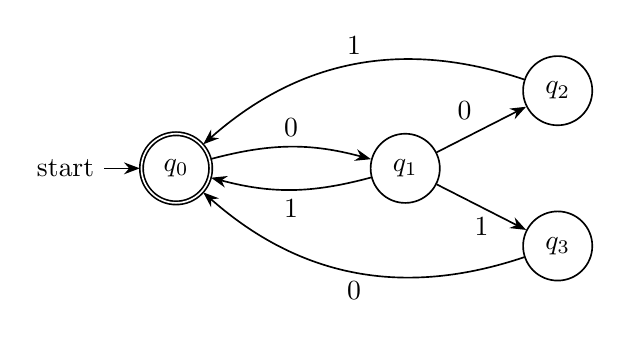
\begin{tikzpicture}[->,>=Stealth,auto,semithick,node distance=2.0cm]
      \node[state,initial,accepting] (q0) {$q_0$};
      \node[state,right=of q0] (q1) {$q_1$};
      \node[state,above right=0.35cm and 1.3cm of q1] (q2) {$q_2$};
      \node[state,below right=0.35cm and 1.3cm of q1] (q3) {$q_3$};
      \path (q0) edge[bend left=15] node {$0$} (q1)
        (q1) edge[bend left=15] node {$1$} (q0)
        (q1) edge node {$0$} (q2)
        (q1) edge node[below] {$1$} (q3)
        (q2) edge[bend right=30] node[above] {$1$} (q0)
        (q3) edge[bend left=30] node[below] {$0$} (q0);
    \end{tikzpicture}
  \end{center}
  \pause
  From $q_1$, input $1$ may finish $01$ or continue toward $010$.
  This nondeterminism is essential to this particular prefix-sharing design.
  The three first-return paths spell exactly $01$, $001$, and $010$.
  \par\smallskip
  {\scriptsize Adapted from Sipser's Exercise~1.17, identified
  in~\cite{sheard}. This is a compact NFA, not the literal Thompson output.}
\end{frame}

\begin{frame}{Solution: Reachable Subsets and a Complete DFA}
  \small
  Use the NFA on the preceding slide. For a subset $Q'$, take the union of
  all possible next states. A subset accepts exactly when it contains $q_0$.
  \pause
  \begin{center}
    \begin{tabular}{c|l|cc|c}
      DFA state & NFA subset & on $0$ & on $1$ & Accept? \\
      \hline
      $A$ (start) & $\{q_0\}$     & $B$ & $\bot$ & yes \\
      $B$ & $\{q_1\}$           & $C$ & $D$ & no \\
      $C$ & $\{q_2\}$           & $\bot$ & $A$ & no \\
      $D$ & $\{q_0,q_3\}$       & $E$ & $\bot$ & yes \\
      $E$ & $\{q_0,q_1\}$       & $F$ & $D$ & yes \\
      $F$ & $\{q_1,q_2\}$       & $C$ & $D$ & no \\
      $\bot$ & $\emptyset$      & $\bot$ & $\bot$ & no
    \end{tabular}
  \end{center}
  \pause
  All seven subsets are reachable, for example by
  $\varepsilon,0,00,01,010,0100,1$, respectively.
  \begin{exampleblock}{Check the boundary ambiguity}
    After $01$, both $q_0$ and $q_3$ are possible. On the next $0$, one
    computation starts a new factor and another finishes $010$:
    $D\xrightarrow{0}E$. Keeping only one computation would lose words.
  \end{exampleblock}
  Reachable does not mean minimal; minimization is a separate task.
\end{frame}

\begin{frame}{Challenge: Change the Elimination Order}
  \small
  Return to the odd-number-of-$1$'s DFA, with even state $q_e$ (start),
  odd state $q_o$ (accept), $0$-loops, and $1$-transitions between them.
  \textbf{Now eliminate $q_e$ before $q_o$.}
  \pause
  After adding GNFA boundaries $s,f$, the relevant surviving labels are
  \[
    R_{s,o}=0^*1,\qquad R_{o,o}=0\cup10^*1,\qquad
    R_{o,f}=\varepsilon.
  \]
  Eliminating $q_o$ next gives
  \[
    0^*1(0\cup10^*1)^*.
  \]
  \pause
  \begin{block}{Why it agrees with the main lecture}
    The main order gave $(0\cup10^*1)^*10^*$. In both expressions there
    is one unpaired $1$ and zero or more pairs of $1$'s, with arbitrary
    zeros. Any word with an odd number of $1$'s admits either grouping.
  \end{block}
  This is a language-equivalence argument, \emph{not} a claim that
  concatenation is commutative. Elimination order changes the expression,
  not the recognized language.
\end{frame}

\begin{frame}{Challenge: Solve a Regular Grammar Algebraically}
  \small
  \textbf{Task.} Find an RE for this right-linear grammar:
  \[
    S\to abA\mid B,\qquad A\to aS\mid\varepsilon,\qquad
    B\to bB\mid\varepsilon.
  \]
  Let $X_S,X_A,X_B$ denote the terminal languages generated by the variables.
  \pause
  \[
    X_B=b^*,\qquad X_A=aX_S\cup\varepsilon,\qquad
    X_S=abX_A\cup X_B=abaX_S\cup ab\cup b^*.
  \]
  Arden's lemma applies because $\varepsilon\notin\{aba\}$, giving
  \[
    X_S=(aba)^*(ab\cup b^*).
  \]
  \pause
  \textbf{Independent check.} Each return
  $S\Rightarrow abA\Rightarrow abaS$ contributes $aba$. Termination
  contributes either $ab$ via $A\to\varepsilon$, or a word of $b^*$
  via $S\to B$. These are all possible choices, proving both inclusions.
  \par\smallskip
  {\scriptsize Original synthesis exercise combining Linz's regular-grammar
  constructions with Arden's lemma; unit and empty productions matter.}
\end{frame}

\subsection{Alternative Constructions and Further Observations}

\begin{frame}{Brzozowski Derivatives: Reading One Symbol}
  \small
  The derivative $D_a(R)$ describes the possible suffixes after reading $a$:
  \[
    L(D_a(R))=\{z:az\in L(R)\}.
  \]
  Recall that $\nu(R)$ means $\varepsilon\in L(R)$.
  \pause
  \[
    \begin{aligned}
      D_a(\emptyset)&=D_a(\varepsilon)=\emptyset,\\
      D_a(b)&=\begin{cases}\varepsilon&b=a,\\\emptyset&b\ne a,\end{cases}\\
      D_a(R\cup S)&=D_a(R)\cup D_a(S),\\
      D_a(RS)&=D_a(R)S\cup
        \begin{cases}D_a(S)&\nu(R),\\\emptyset&\text{otherwise},\end{cases}\\
      D_a(R^*)&=D_a(R)R^*.
    \end{aligned}
  \]
  \pause
  In concatenation, $a$ is consumed in the first factor unless that factor
  contributes $\varepsilon$. For membership, differentiate along the input
  and test whether the final expression is nullable. See~\cite{brzozowski}.
\end{frame}

\begin{frame}{Worked Derivatives: A DFA for the Earlier RE}
  \small
  Let $R=(ab\cup a)^*$ and $T=(b\cup\varepsilon)R$.
  Simplifying derivatives gives the following complete transition table:
  \begin{center}
    \begin{tabular}{c|cc|c}
      Expression state & on $a$ & on $b$ & Nullable (accepting)? \\
      \hline
      $R$ (start) & $T$ & $\emptyset$ & yes \\
      $T$ & $T$ & $R$ & yes \\
      $\emptyset$ & $\emptyset$ & $\emptyset$ & no
    \end{tabular}
  \end{center}
  \pause
  For example,
  \[
    D_a(R)=(b\cup\varepsilon)R=T,\quad
    D_b(T)=\varepsilon R\cup D_b(R)=R.
  \]
  Thus $R\xrightarrow{a}T\xrightarrow{b}R\xrightarrow{a}T$ accepts $aba$,
  whereas $R\xrightarrow{a}T\xrightarrow{b}R\xrightarrow{b}\emptyset$
  rejects $abb$.
  \pause
  \begin{alertblock}{Implementation qualification}
    Equivalent expressions need not look identical. A general derivative
    construction needs normalization or an equivalence-aware representation;
    blindly treating every new syntax tree as a distinct state is not enough.
  \end{alertblock}
\end{frame}

\begin{frame}{Glushkov's Position Automaton: An Epsilon-Free Route}
  \small
  Mark the $m$ terminal occurrences of an RE with distinct positions.
  The \textbf{position automaton} has these $m$ states plus a new start $0$.
  \begin{itemize}
    \item $\mathrm{First}$: positions that can begin a nonempty marked word.
    \item $\mathrm{Last}$: positions that can end a nonempty marked word.
    \item $\mathrm{Follow}(i)$: positions that can immediately follow $i$.
  \end{itemize}
  \pause
  \begin{block}{Construction}
    Add $0\xrightarrow{\mathrm{symbol}(j)}j$ for $j\in\mathrm{First}$,
    and $i\xrightarrow{\mathrm{symbol}(j)}j$ for
    $j\in\mathrm{Follow}(i)$. Accept at every position in $\mathrm{Last}$;
    also accept at $0$ exactly when the RE is nullable.
  \end{block}
  \pause
  The invariant records the last matched occurrence. The marked RE's
  first/follow/last constraints characterize its nonempty words; removing
  position indices recovers the original language.
  \par\smallskip
  No $\varepsilon$-edges are needed, but the number of edges can be quadratic
  in $m$; fewer states does not automatically mean less storage.
  See~\cite{allauzen-mohri} for this construction and related automata.
\end{frame}

\begin{frame}{Worked Position Automaton: The Earlier RE}
  \small
  Mark the earlier RE as $(a_1b_2\cup a_3)^*$. The indices distinguish
  occurrences of $a$, not different alphabet symbols.
  \[
    \mathrm{First}=\{1,3\},\qquad \mathrm{Last}=\{2,3\},
  \]
  \[
    \mathrm{Follow}(1)=\{2\},\qquad
    \mathrm{Follow}(2)=\mathrm{Follow}(3)=\{1,3\}.
  \]
  \pause
  \begin{center}
    \begin{tabular}{c|cc|c}
      State & on $a$ & on $b$ & Accepting? \\
      \hline
      $0$ (start) & $\{1,3\}$ & $\emptyset$ & yes \\
      $1$ & $\emptyset$ & $\{2\}$ & no \\
      $2$ & $\{1,3\}$ & $\emptyset$ & yes \\
      $3$ & $\{1,3\}$ & $\emptyset$ & yes
    \end{tabular}
  \end{center}
  \pause
  Both $0\xrightarrow{a}3$ and $0\xrightarrow{a}1\xrightarrow{b}2$
  accept a factor. Star contributes the transitions back to first positions.
  Compare: the Thompson construction uses fragment boundaries; the derivative
  DFA stores residual expressions; this NFA stores matched positions.
\end{frame}

\begin{frame}{Observation: Ambiguity in a Regular Grammar}
  \small
  Informally, a grammar is \textbf{ambiguous} if a word has two different
  parse structures (here, two distinct production-choice sequences).
  Consider the right-linear grammar
  \[
    S\to aS\mid A,\qquad A\to aA\mid\varepsilon.
  \]
  For example, $a$ has the derivations
  \[
    S\Rightarrow aS\Rightarrow aA\Rightarrow a,
    \qquad S\Rightarrow A\Rightarrow aA\Rightarrow a.
  \]
  \pause
  Its language is $a^*$, which also has the unambiguous grammar
  $S\to aS\mid\varepsilon$. For $a^n$, the first grammar has $n+1$
  choices for when to switch from $S$ to $A$.
  \begin{block}{Why every regular language has an unambiguous grammar}
    Convert a DFA to a right-linear grammar. Each input symbol forces the
    next state-variable, and only the final accepting state can terminate
    the derivation. The unique accepting path gives a unique derivation.
  \end{block}
  Ambiguity concerns the chosen description, not regularity of its language.
  Formal parse-tree definitions belong to the CFG slide set.
\end{frame}

\subsection{References}

\begin{frame}{References: Enrichment and Exercise Sources}
  \footnotesize
  \setbeamertemplate{bibliography item}[text]
  \begin{thebibliography}{9}
    \bibitem[B64]{brzozowski}
      Janusz A. Brzozowski,
      \href{https://doi.org/10.1145/321239.321249}
      {\emph{Derivatives of Regular Expressions}},
      Journal of the ACM 11(4), 1964, pp.\ 481--494.
    \bibitem[AM06]{allauzen-mohri}
      Cyril Allauzen and Mehryar Mohri,
      \href{https://cs.nyu.edu/media/publications/TR2006-880.pdf}
      {\emph{A Unified Construction of the Glushkov, Follow, and Antimirov
      Automata}}, NYU technical report TR2006-880, 2006.
    \bibitem[PSU13]{sheard}
      Tim Sheard, Portland State University CS~311,
      \href{https://web.cecs.pdx.edu/~sheard/course/CS311/Fall2013/homework/assign3.pdf}
      {\emph{Homework 3}}, October 16, 2013.
      Identifies the Sipser 1.17 and 1.18 problems adapted here.
  \end{thebibliography}
  \begin{block}{Attribution and scope}
    The Sipser challenges have independently worked solutions. The other
    challenges synthesize the RE-design and grammar-conversion themes of
    Linz and Sipser; no unverified textbook exercise numbers are assigned.
  \end{block}
\end{frame}

\begin{frame}{References and Suggested Use}
  \small
  \setbeamertemplate{bibliography item}[text]
  \begin{thebibliography}{9}
    \bibitem[LR23]{linz}
      Peter Linz and Susan H. Rodger,
      \emph{An Introduction to Formal Languages and Automata}, 7th ed.,
      Jones \& Bartlett Learning, 2023.
      Chapter 3: regular languages and regular grammars.
    \bibitem[S13]{sipser}
      Michael Sipser, \emph{Introduction to the Theory of Computation},
      3rd ed., Cengage, 2013. Section 1.3: regular expressions and
      finite-automaton equivalence.
    \bibitem[T68]{thompson}
      Ken Thompson, \emph{Regular Expression Search Algorithm},
      Communications of the ACM 11(6), 1968, pp.\ 419--422.
    \bibitem[C07]{cox}
      Russ Cox, \emph{Regular Expression Matching Can Be Simple And Fast},
      2007. An implementation-oriented explanation of Thompson simulation.
  \end{thebibliography}
  Use the main sequence for the core lecture and the appendix for solutions
  and optional enrichment. Specific adapted exercises are attributed on
  their slides; unnumbered challenges are additional, newly worked practice.
\end{frame}

\end{document}

